\documentclass[10pt]{beamer}

\usetheme[progressbar=frametitle]{metropolis}
\usepackage{appendixnumberbeamer}

\usepackage{booktabs}
\usepackage[scale=2]{ccicons}

\usepackage{pgfplots}
\usepgfplotslibrary{dateplot}

\usepackage{xspace}
\newcommand{\themename}{\textbf{\textsc{metropolis}}\xspace}

\newcommand{\blankline}{\quad\pagebreak[3]}
\newcommand{\halfblankline}{\quad\vspace{-0.5\baselineskip}\pagebreak[3]}

\title{"Small world" dynamics in focused networks}
% \date{\today}
\date{}
\author{David Nield}
\institute{University of California, Berkeley}

% \titlegraphic{\hfill\includegraphics[height=1.5cm]{logo.pdf}}

\begin{document}

\maketitle

\begin{frame}[fragile]{Small Worlds}

\begin{itemize}
\item Travers and Milgram's "Small World" study, average of 5.2 intermediaries (popularized the notion of 6 degrees of separation) \cite{milgram1977}

\halfblankline

\item Replicated in 2003 using a global population and 18 targets in 13 different countries with median path lengths between 5 and 7 \cite{dodds2003}

\halfblankline

\item But how? One avenue: a few weak ties \cite{watts}.

\end{itemize}
\end{frame}

\begin{frame}[fragile]{Intro to Networks}

	\begin{figure}[h]
    \centering
  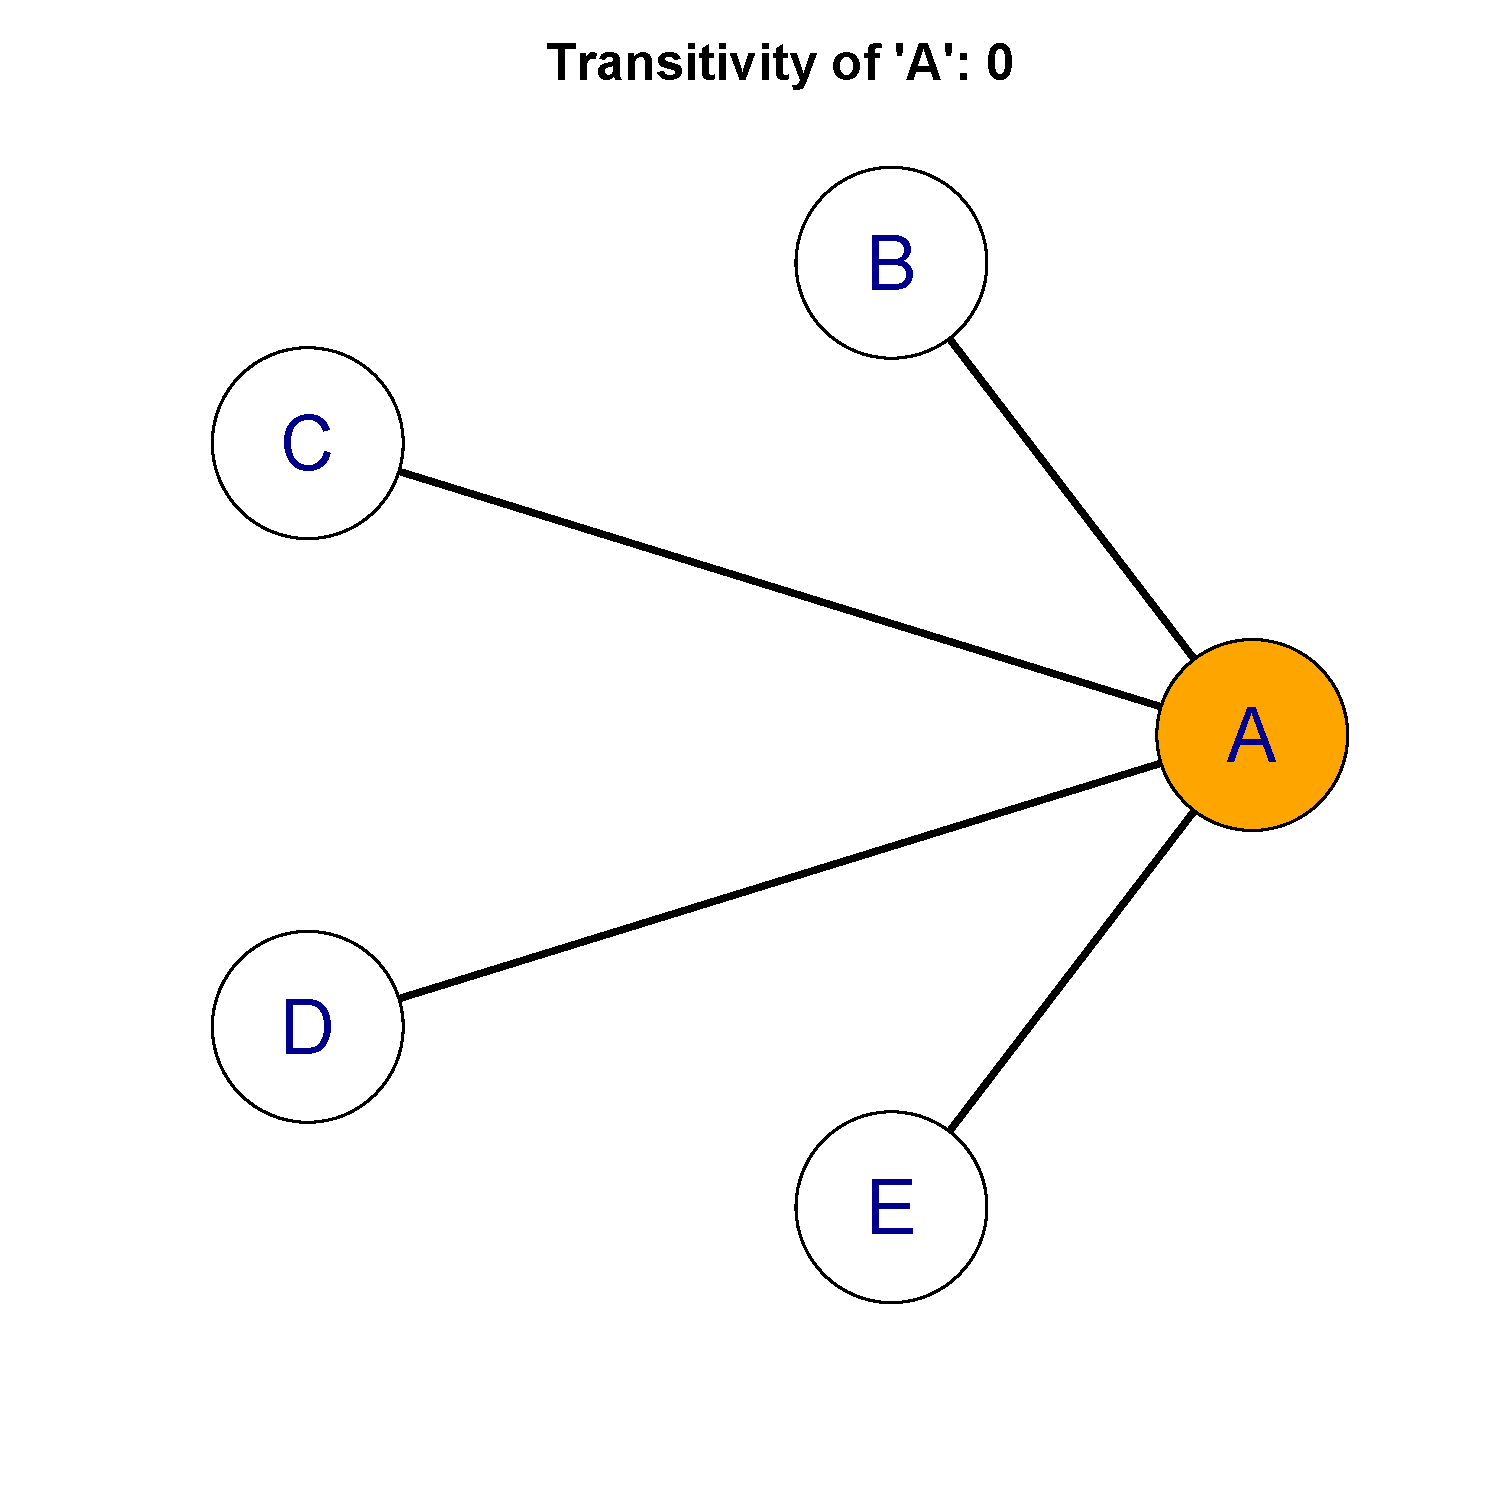
\includegraphics[width = 9cm]{BasicNetworkPlot1.pdf}
  	\end{figure}

\end{frame}

\begin{frame}[fragile]{Intro to Networks}

	\begin{figure}[h]
    \centering
  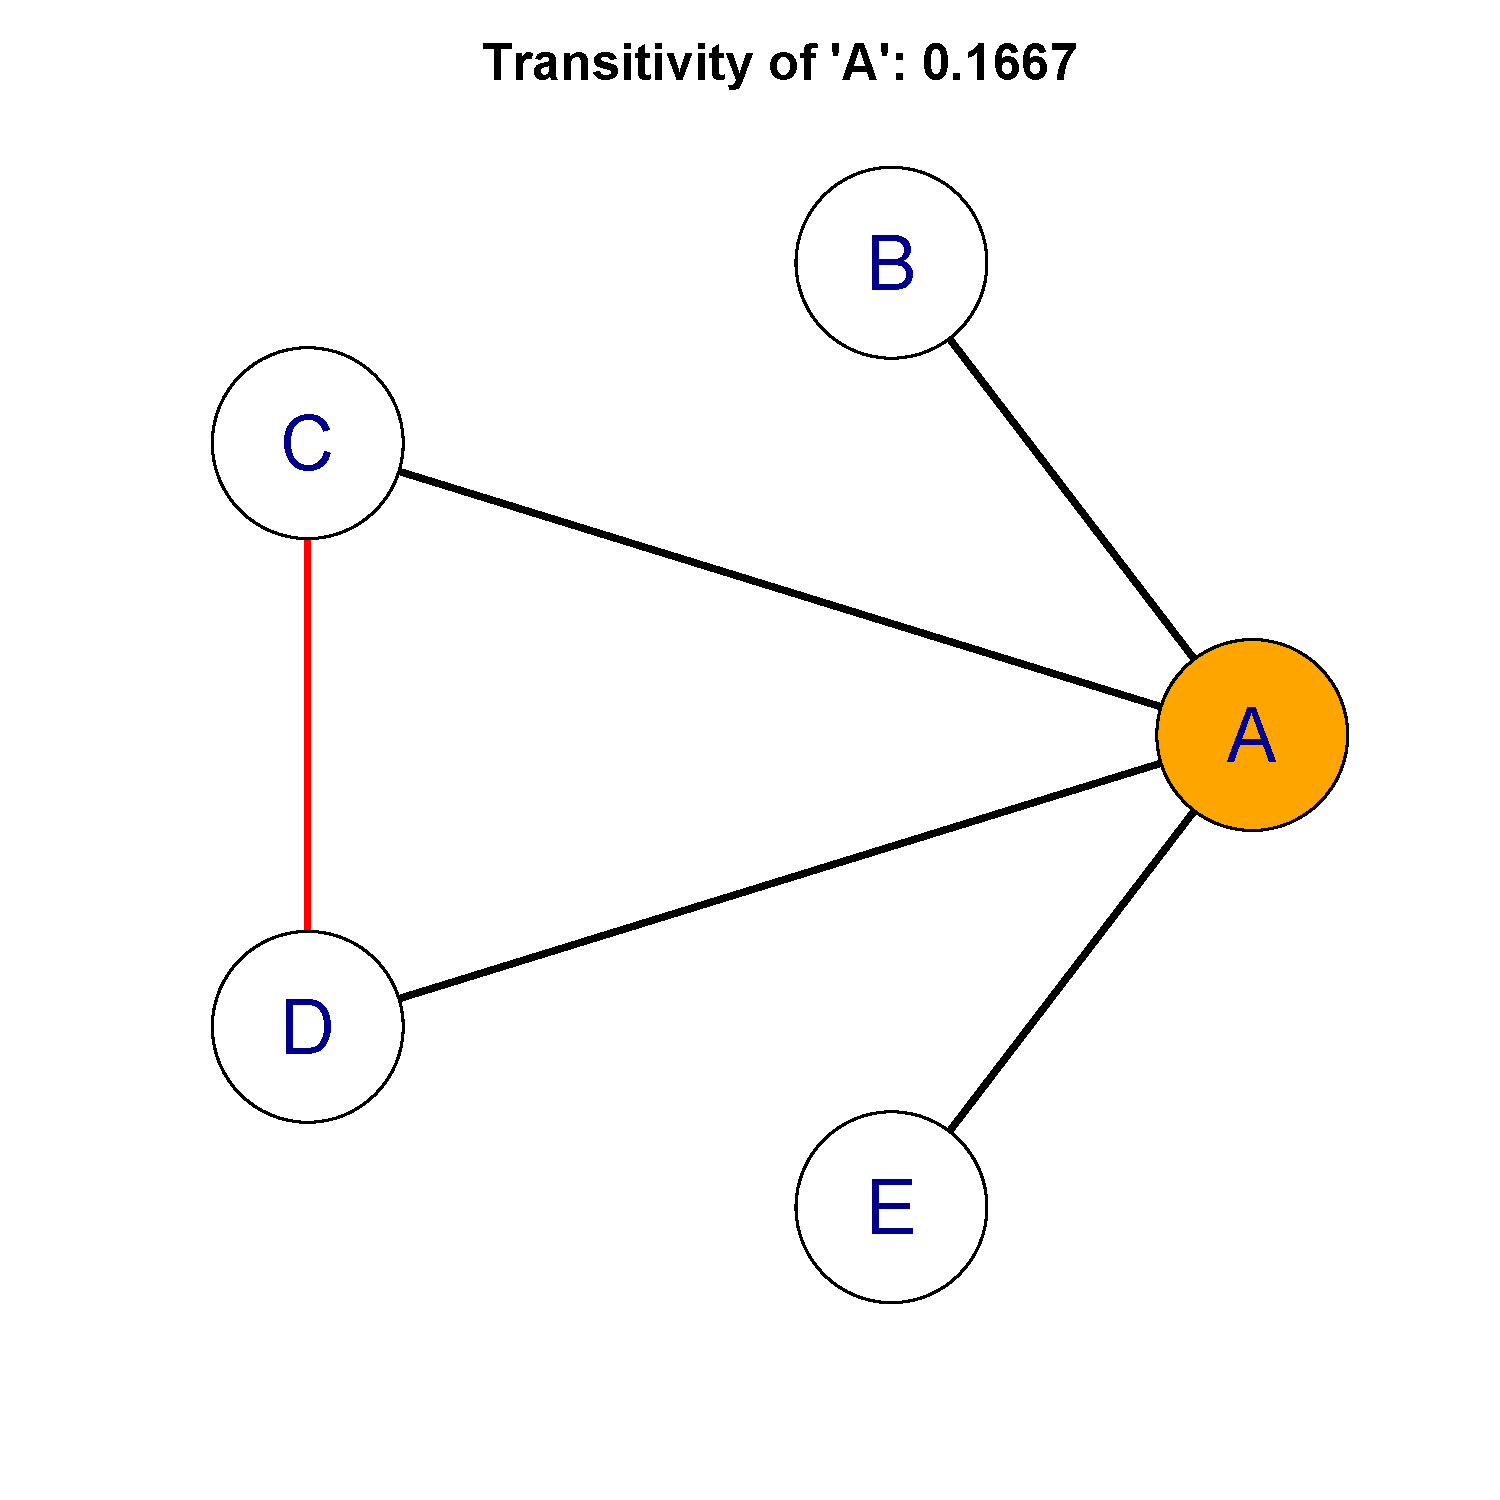
\includegraphics[width = 9cm]{BasicNetworkPlot2.pdf}
  	\end{figure}

\end{frame}

\begin{frame}[fragile]{Small Worlds}

	\begin{figure}[h]
    \centering
  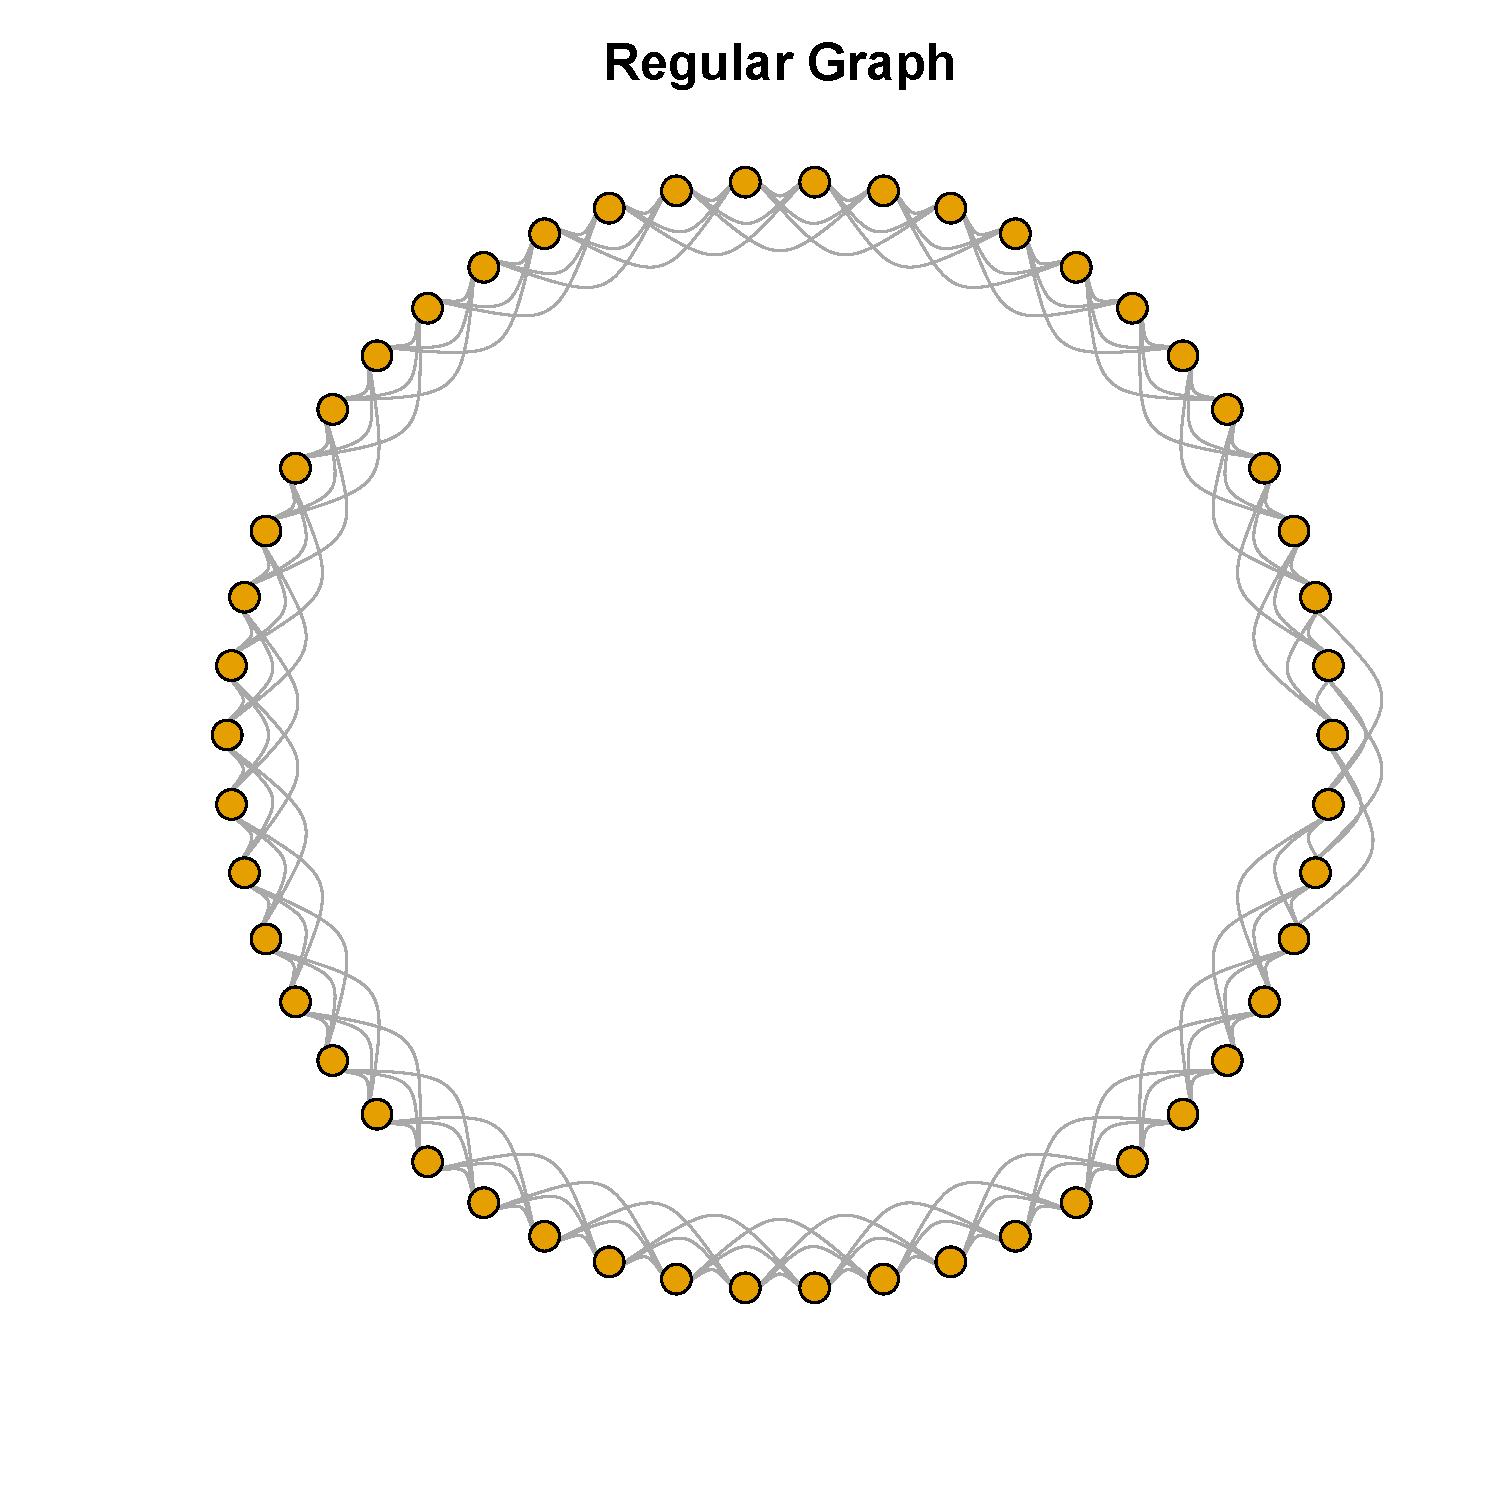
\includegraphics[width = 9cm]{RegularGraph.pdf}
  	\end{figure}

\end{frame}

\begin{frame}[fragile]{Small Worlds}

	\begin{figure}[h]
    \centering
  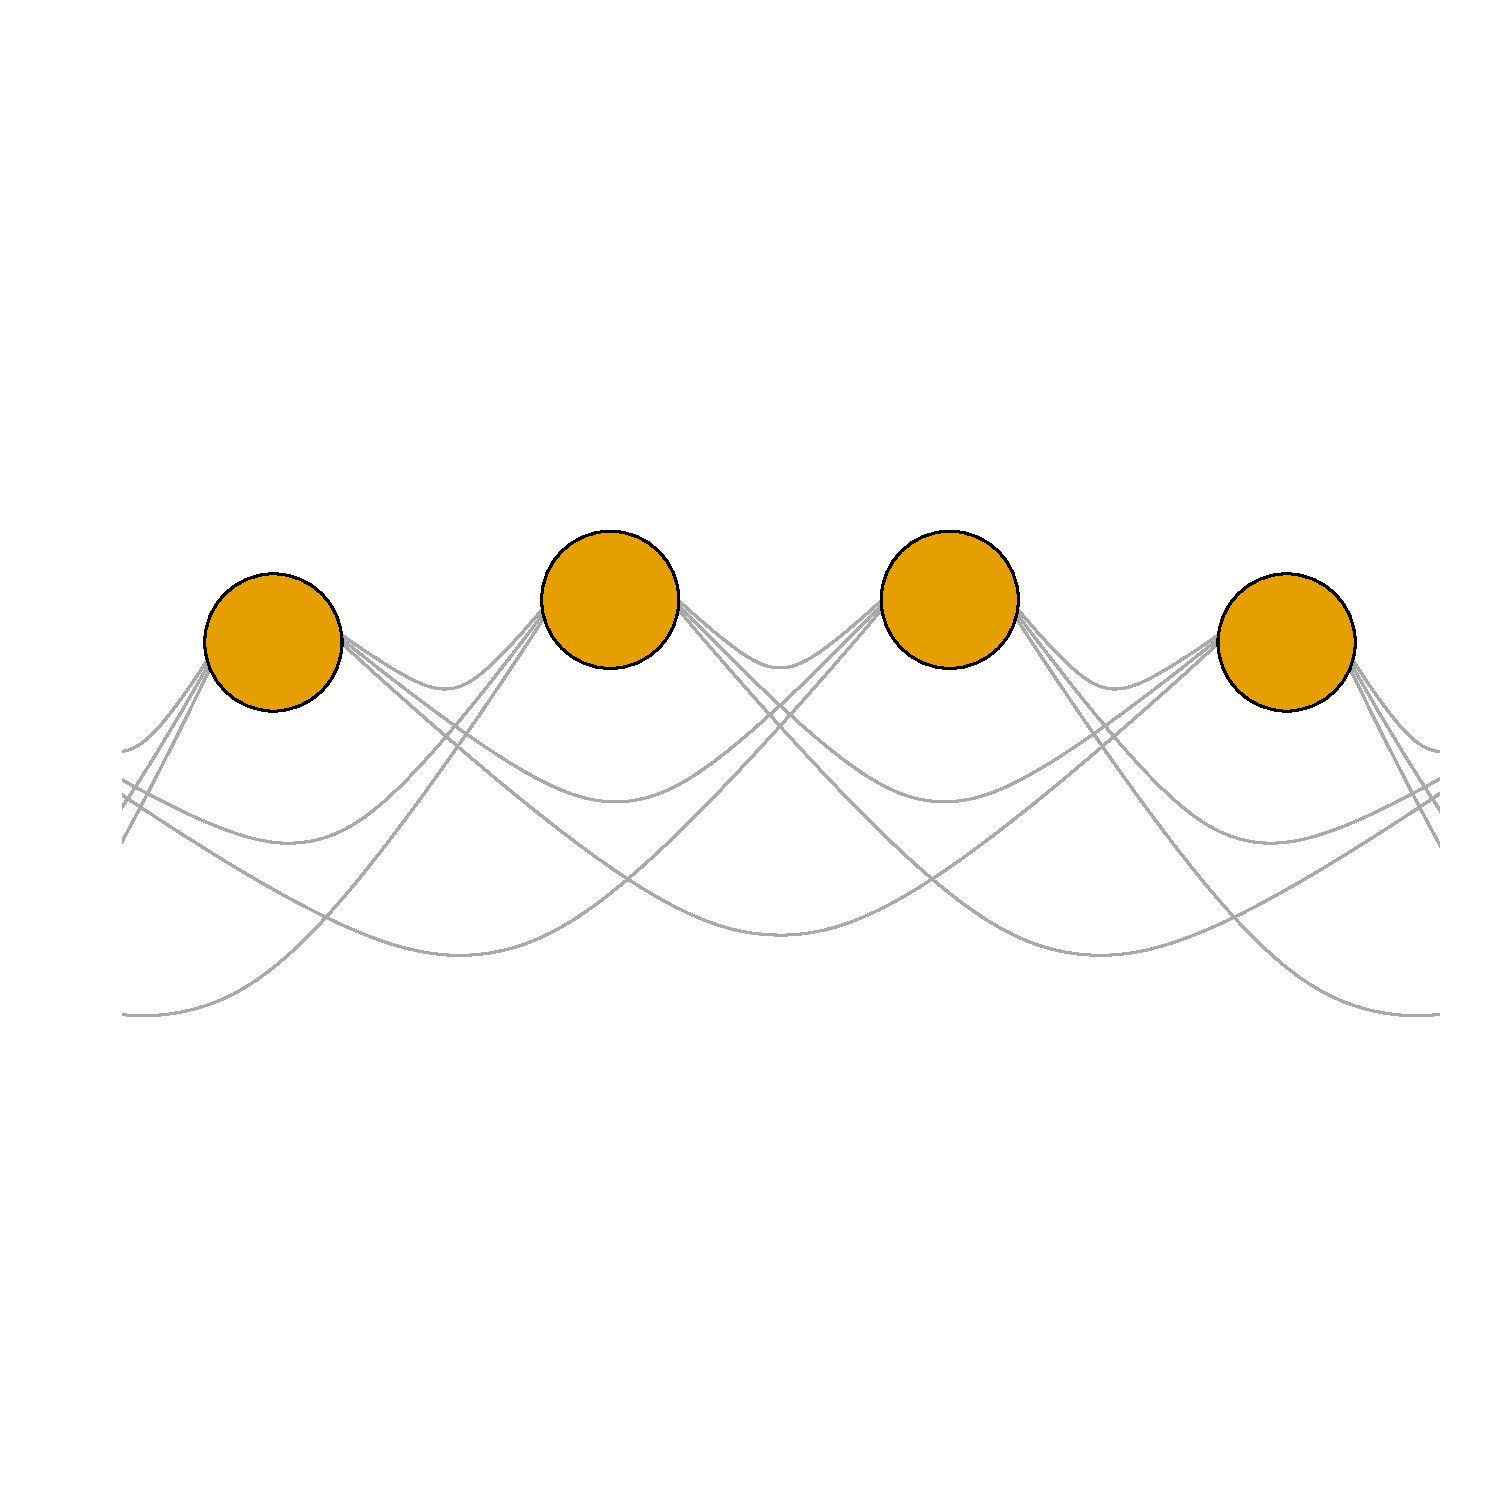
\includegraphics[width = 9cm]{RegularCloseUp.pdf}
  	\end{figure}

\end{frame}

\begin{frame}[fragile]{Small Worlds}

	\begin{figure}[h]
    \centering
  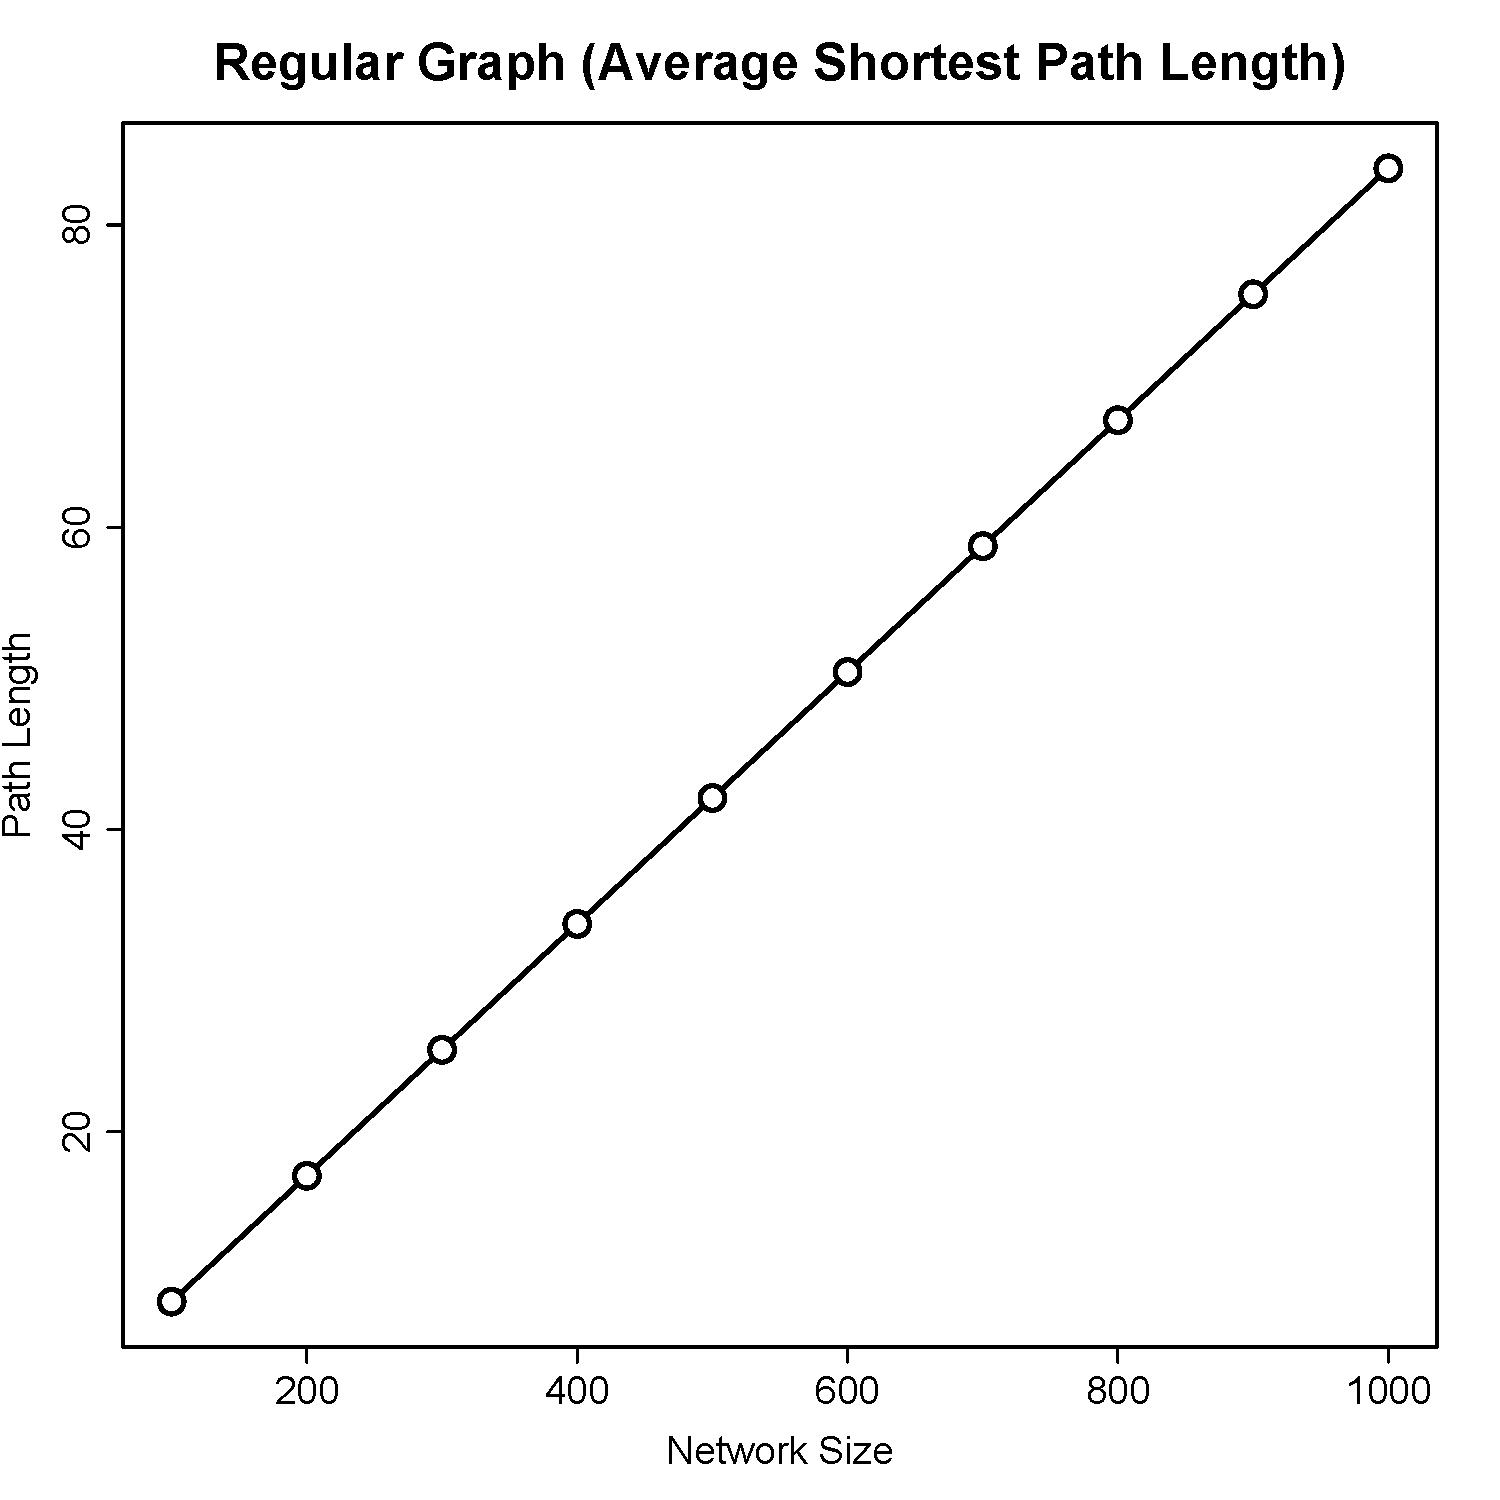
\includegraphics[width = 8.5cm]{RegularPathLength.pdf}
  	\end{figure}

\end{frame}

\begin{frame}[fragile]{Small Worlds}

	\begin{figure}[h]
    \centering
  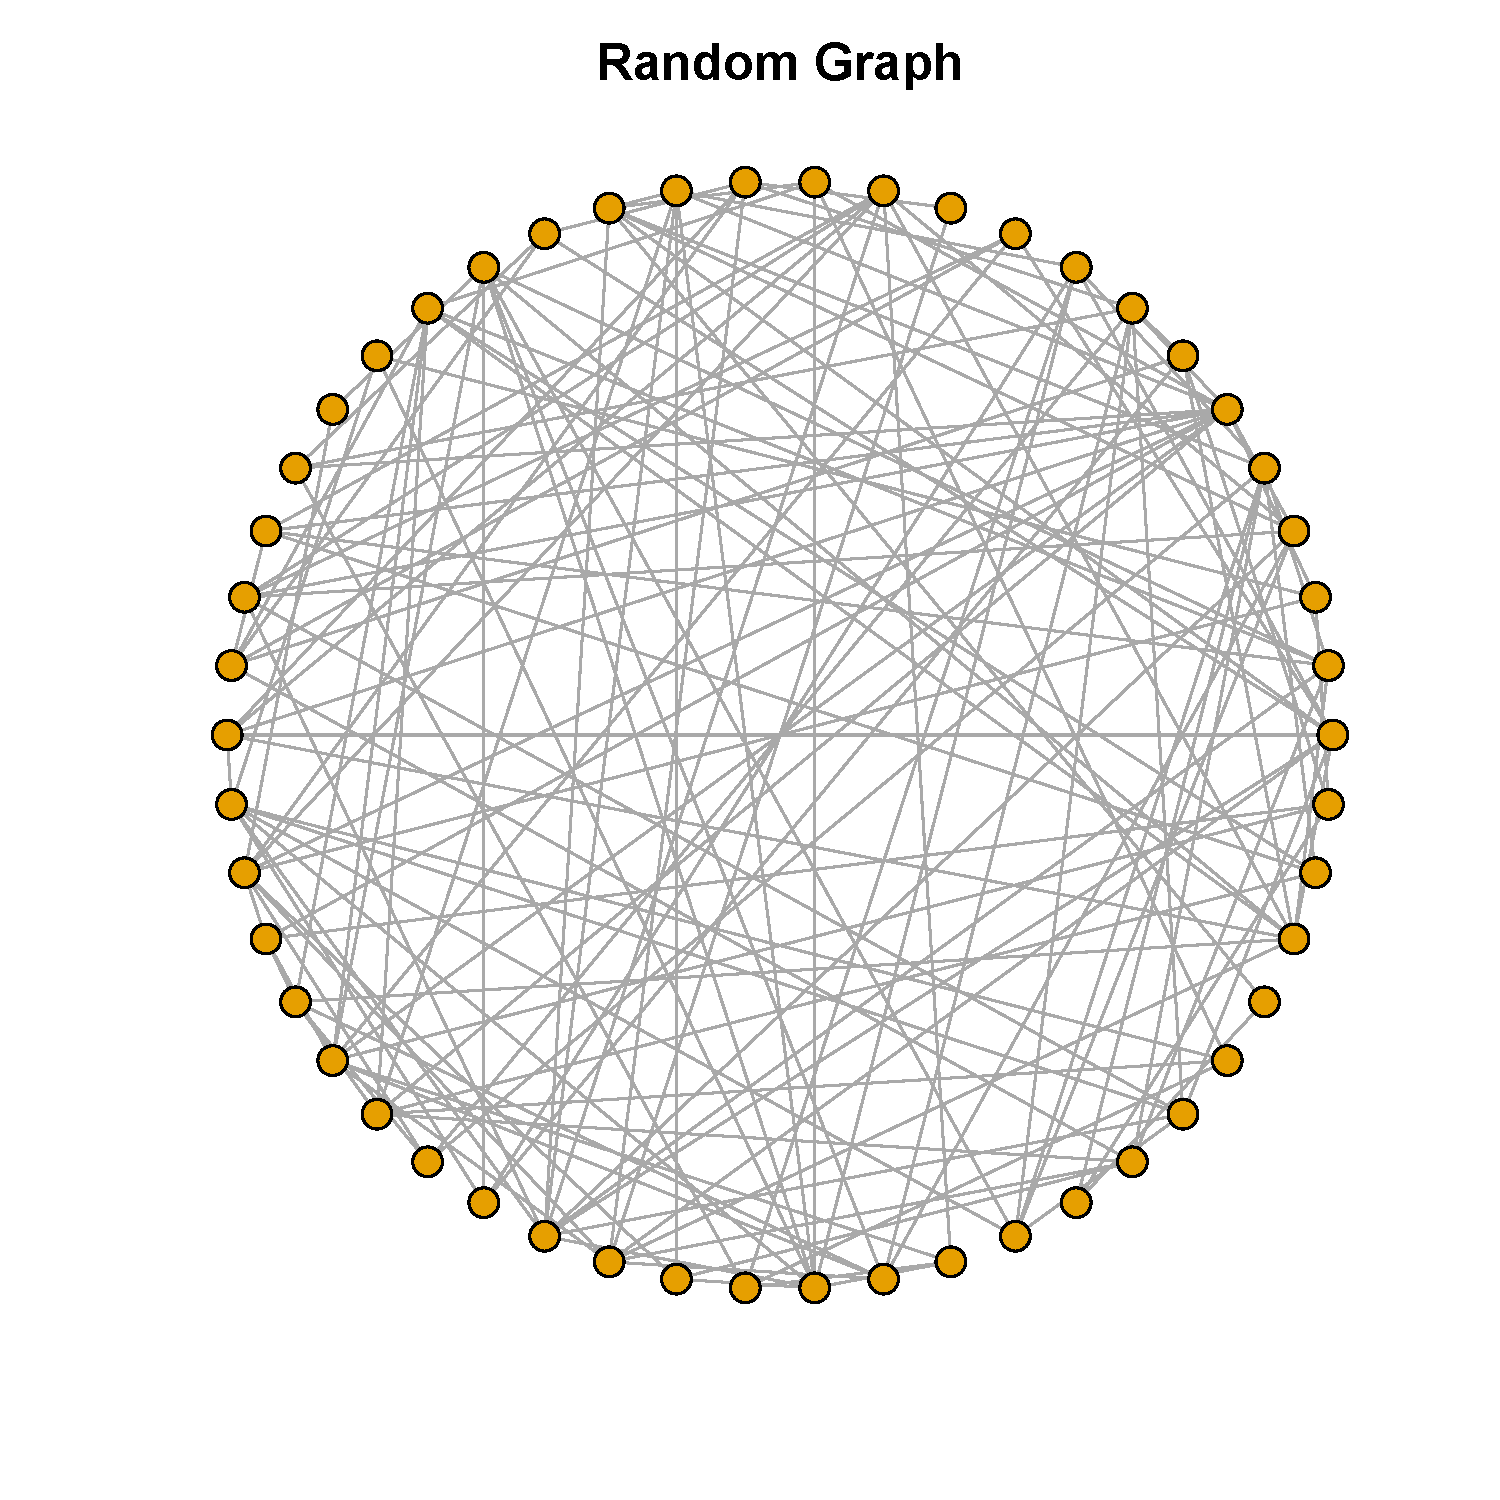
\includegraphics[width = 9cm]{RandomGraph.pdf}
  	\end{figure}

\end{frame}

\begin{frame}[fragile]{Small Worlds}

	\begin{figure}[h]
    \centering
  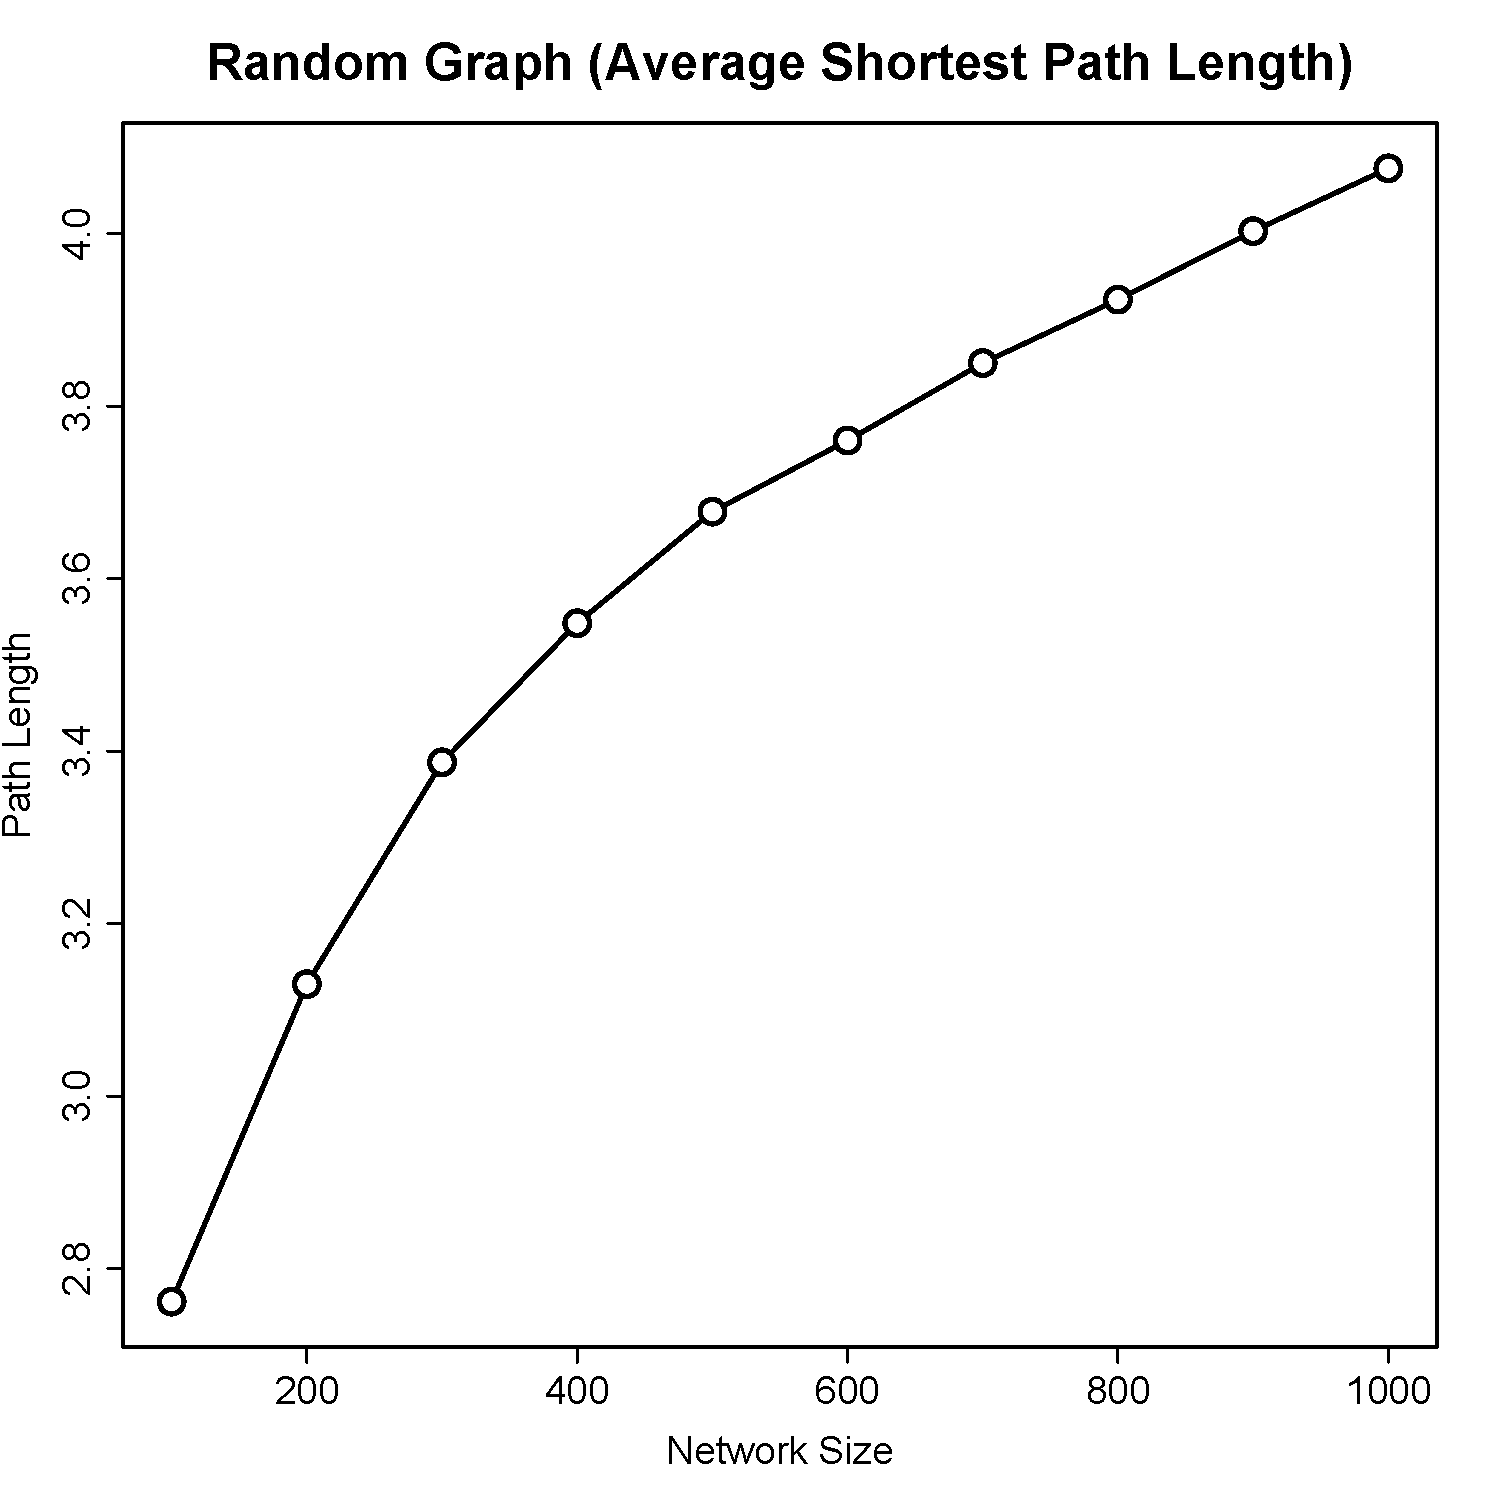
\includegraphics[width = 8.5cm]{RandomPathLength.pdf}
  	\end{figure}

\end{frame}

\begin{frame}[fragile]{Small Worlds}

	\begin{figure}[h]
    \centering
  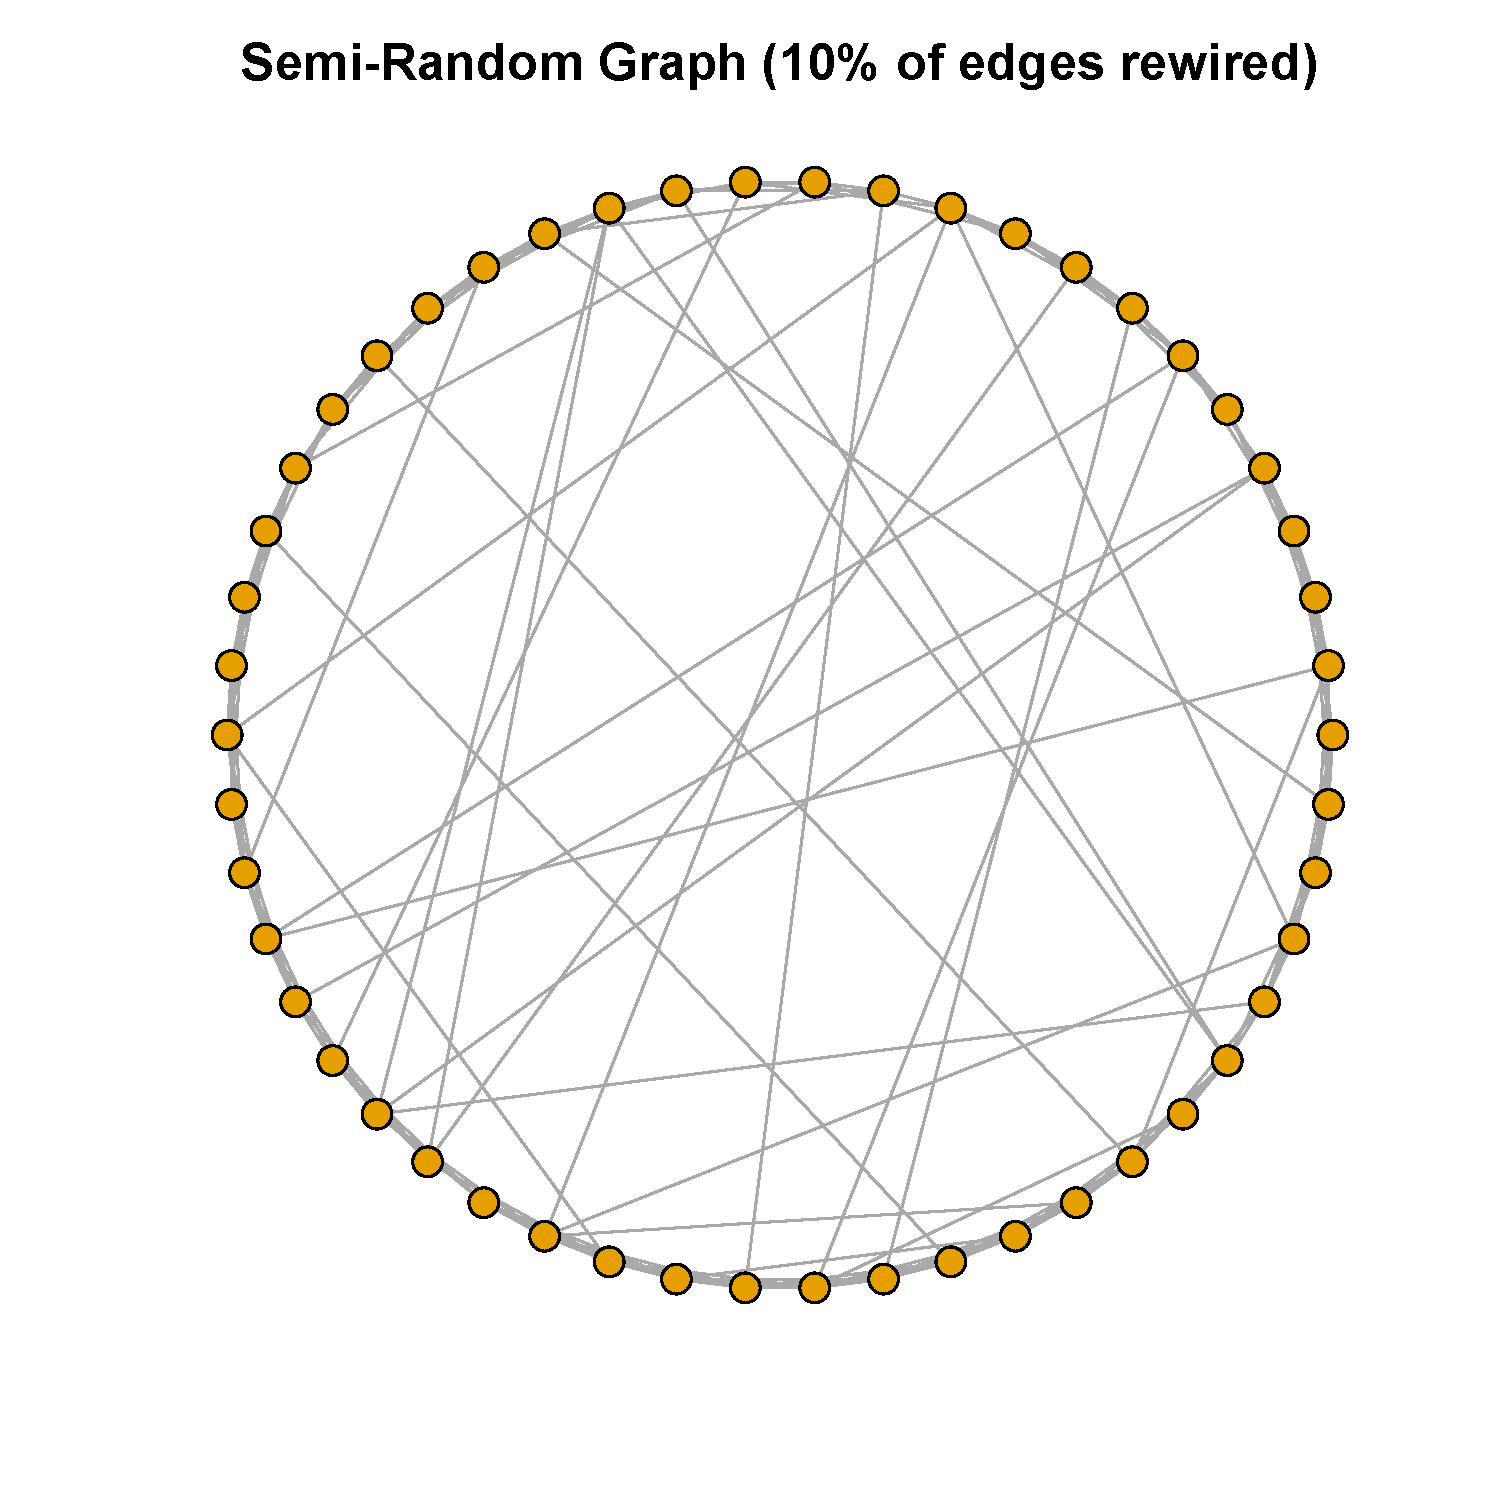
\includegraphics[width = 9cm]{SemiRandomGraph.pdf}
  	\end{figure}

\end{frame}

\begin{frame}[fragile]{Small Worlds}

	\begin{figure}[h]
    \centering
  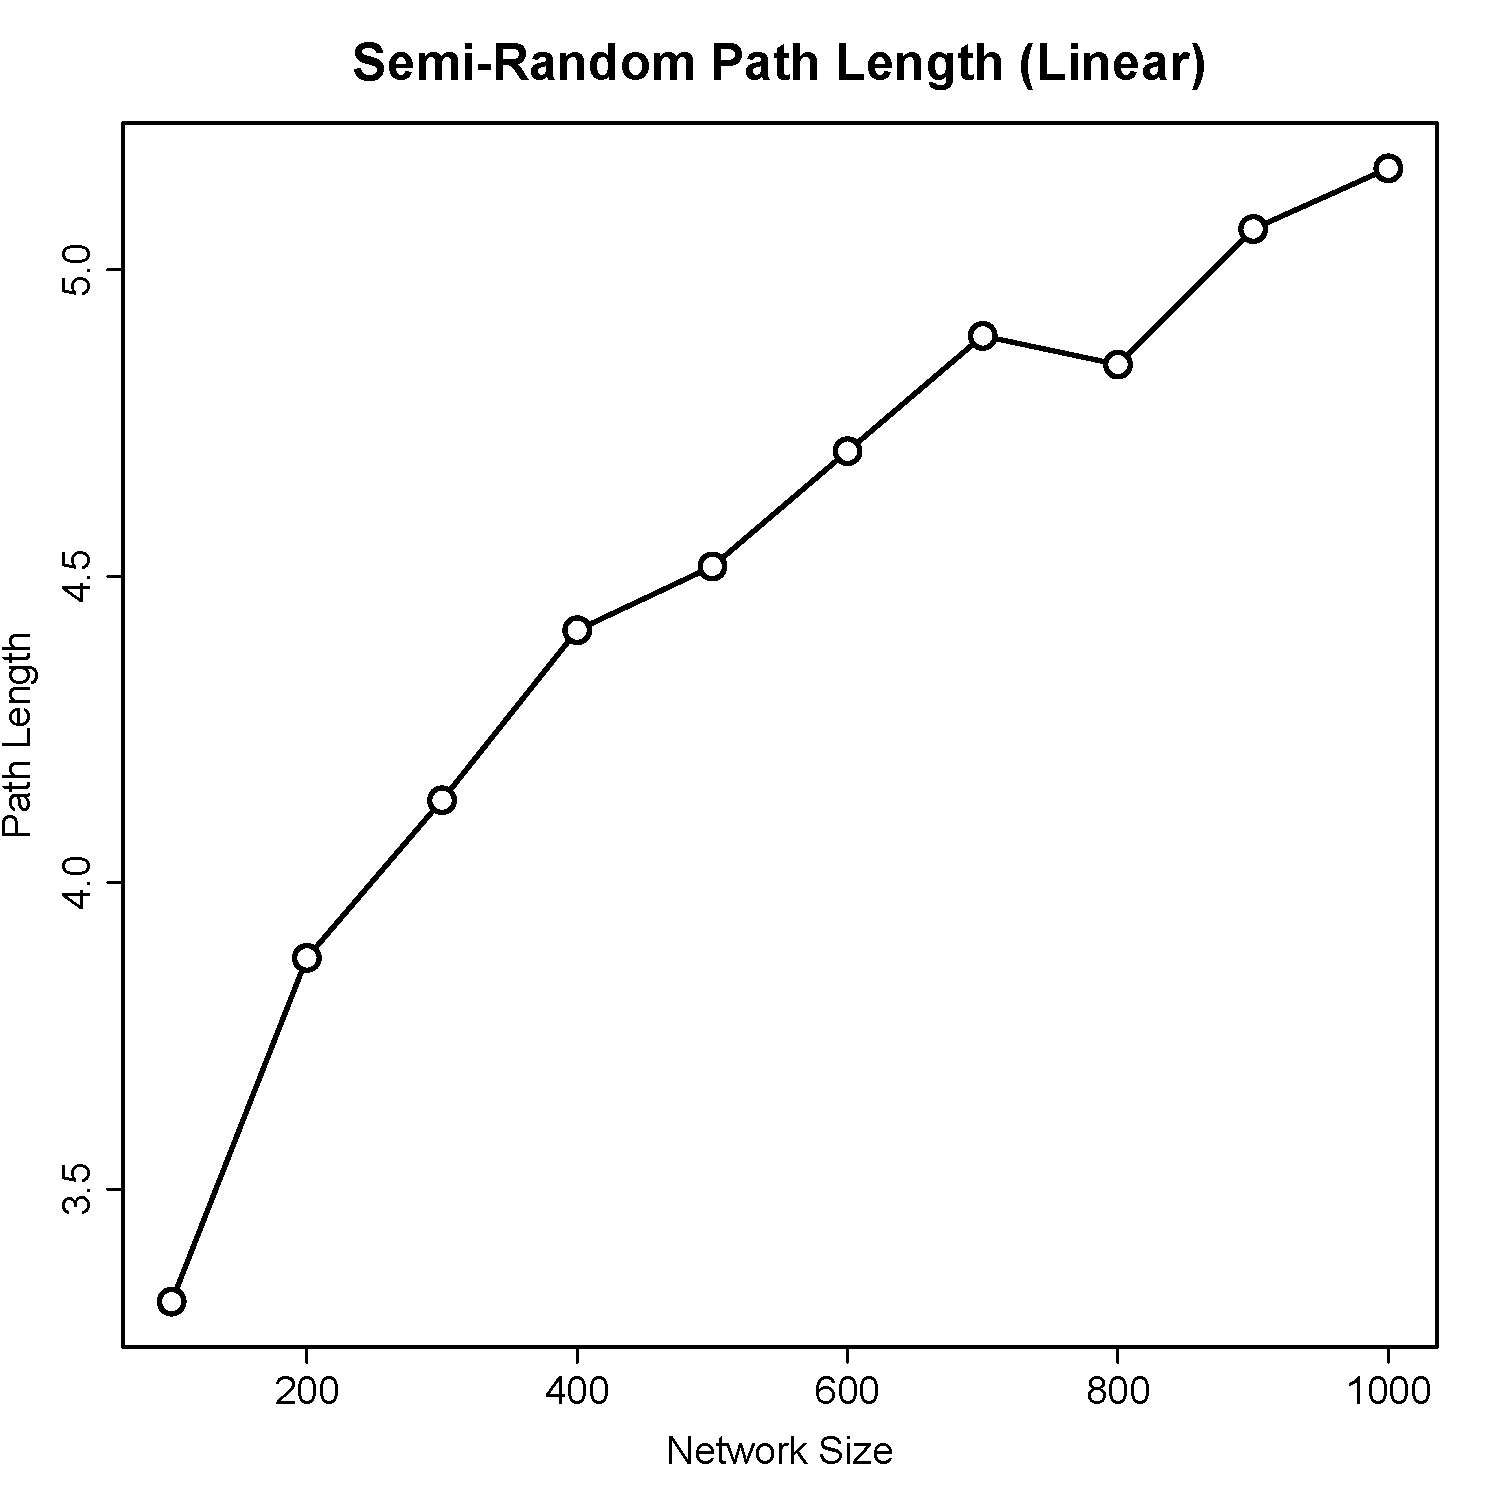
\includegraphics[width = 8.5cm]{SemiRandomPathLength.pdf}
  	\end{figure}

\end{frame}

\begin{frame}[fragile]{Small Worlds}

	\begin{figure}[h]
    \centering
  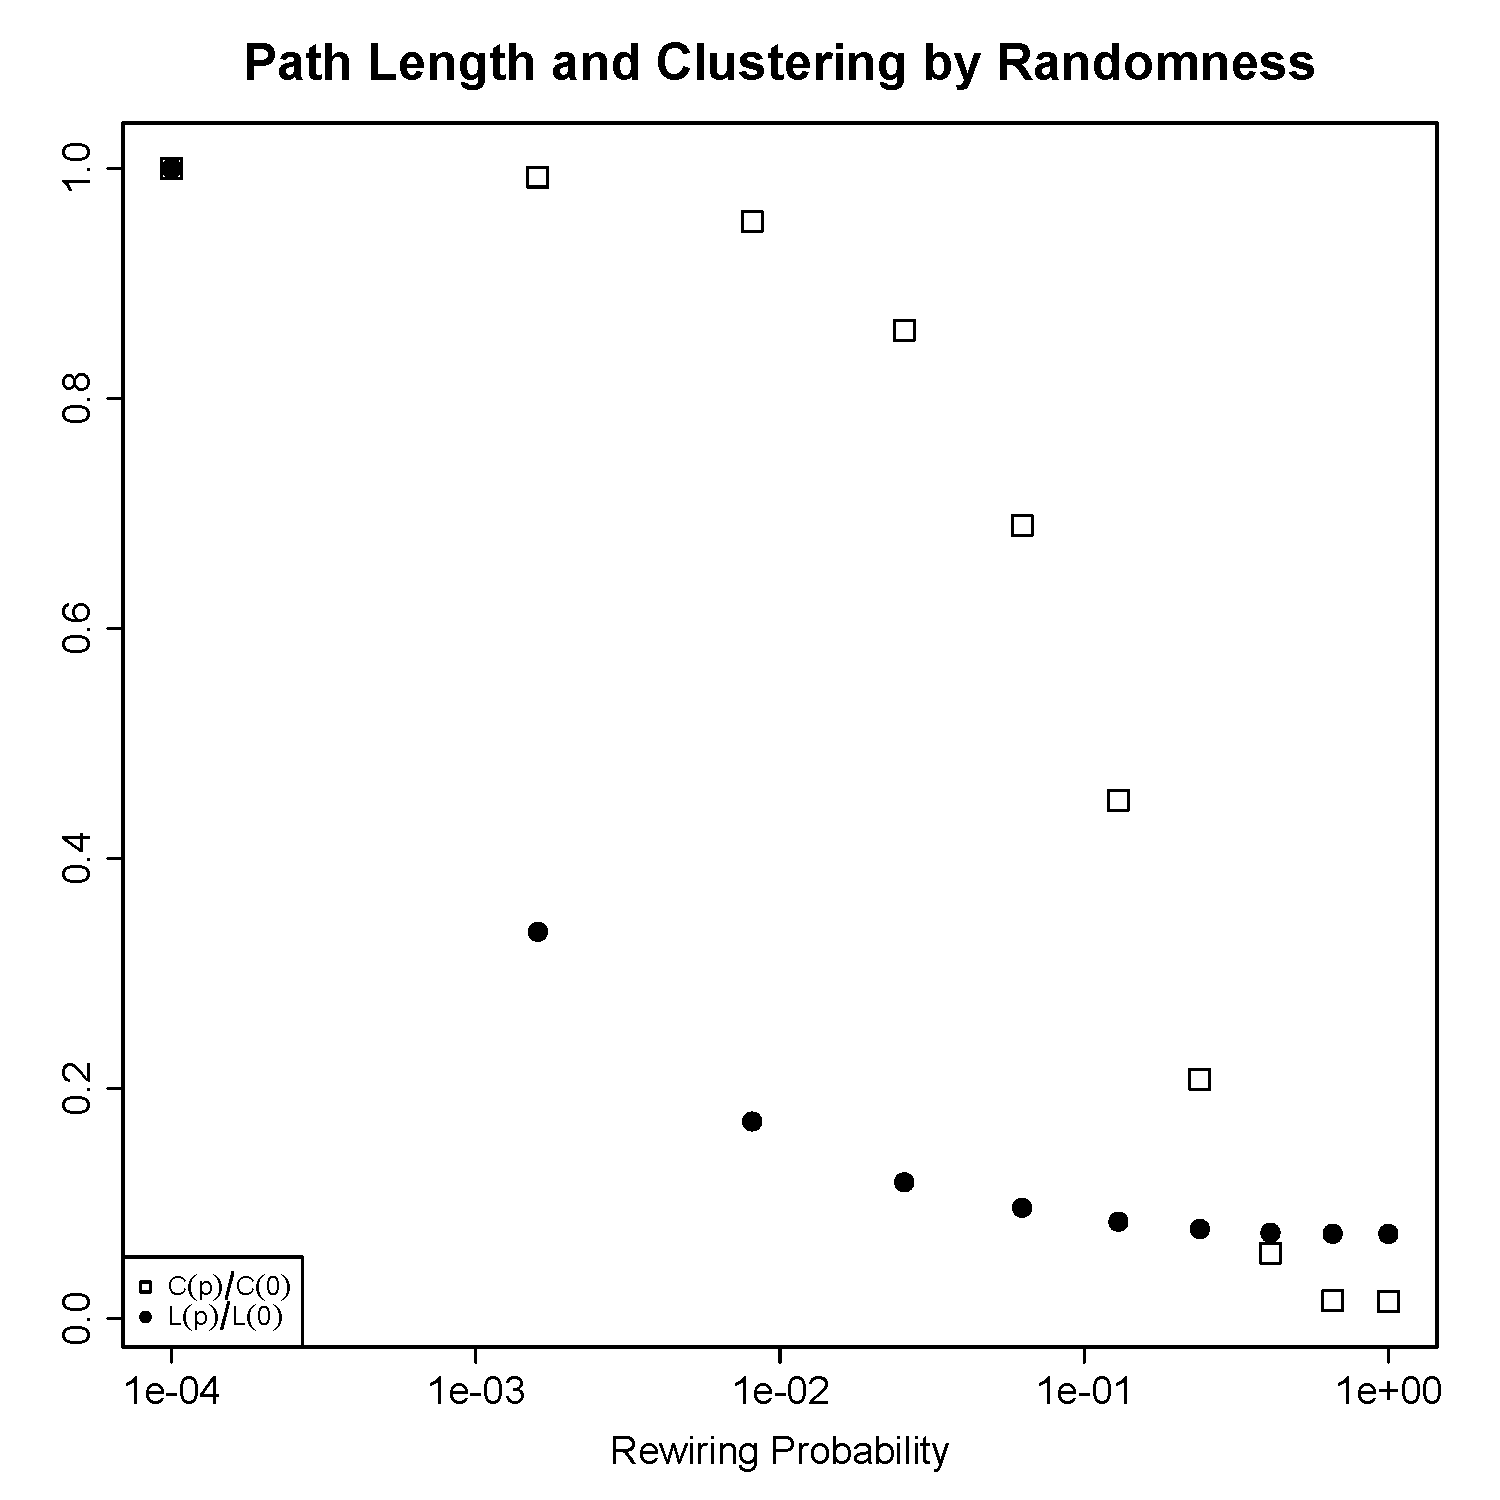
\includegraphics[width = 8.5cm]{WattsStrogatzPlot.pdf}
  	\end{figure}

\end{frame}

\begin{frame}[fragile]{Small Worlds with Focuses}

	\begin{figure}[h]
    \centering
  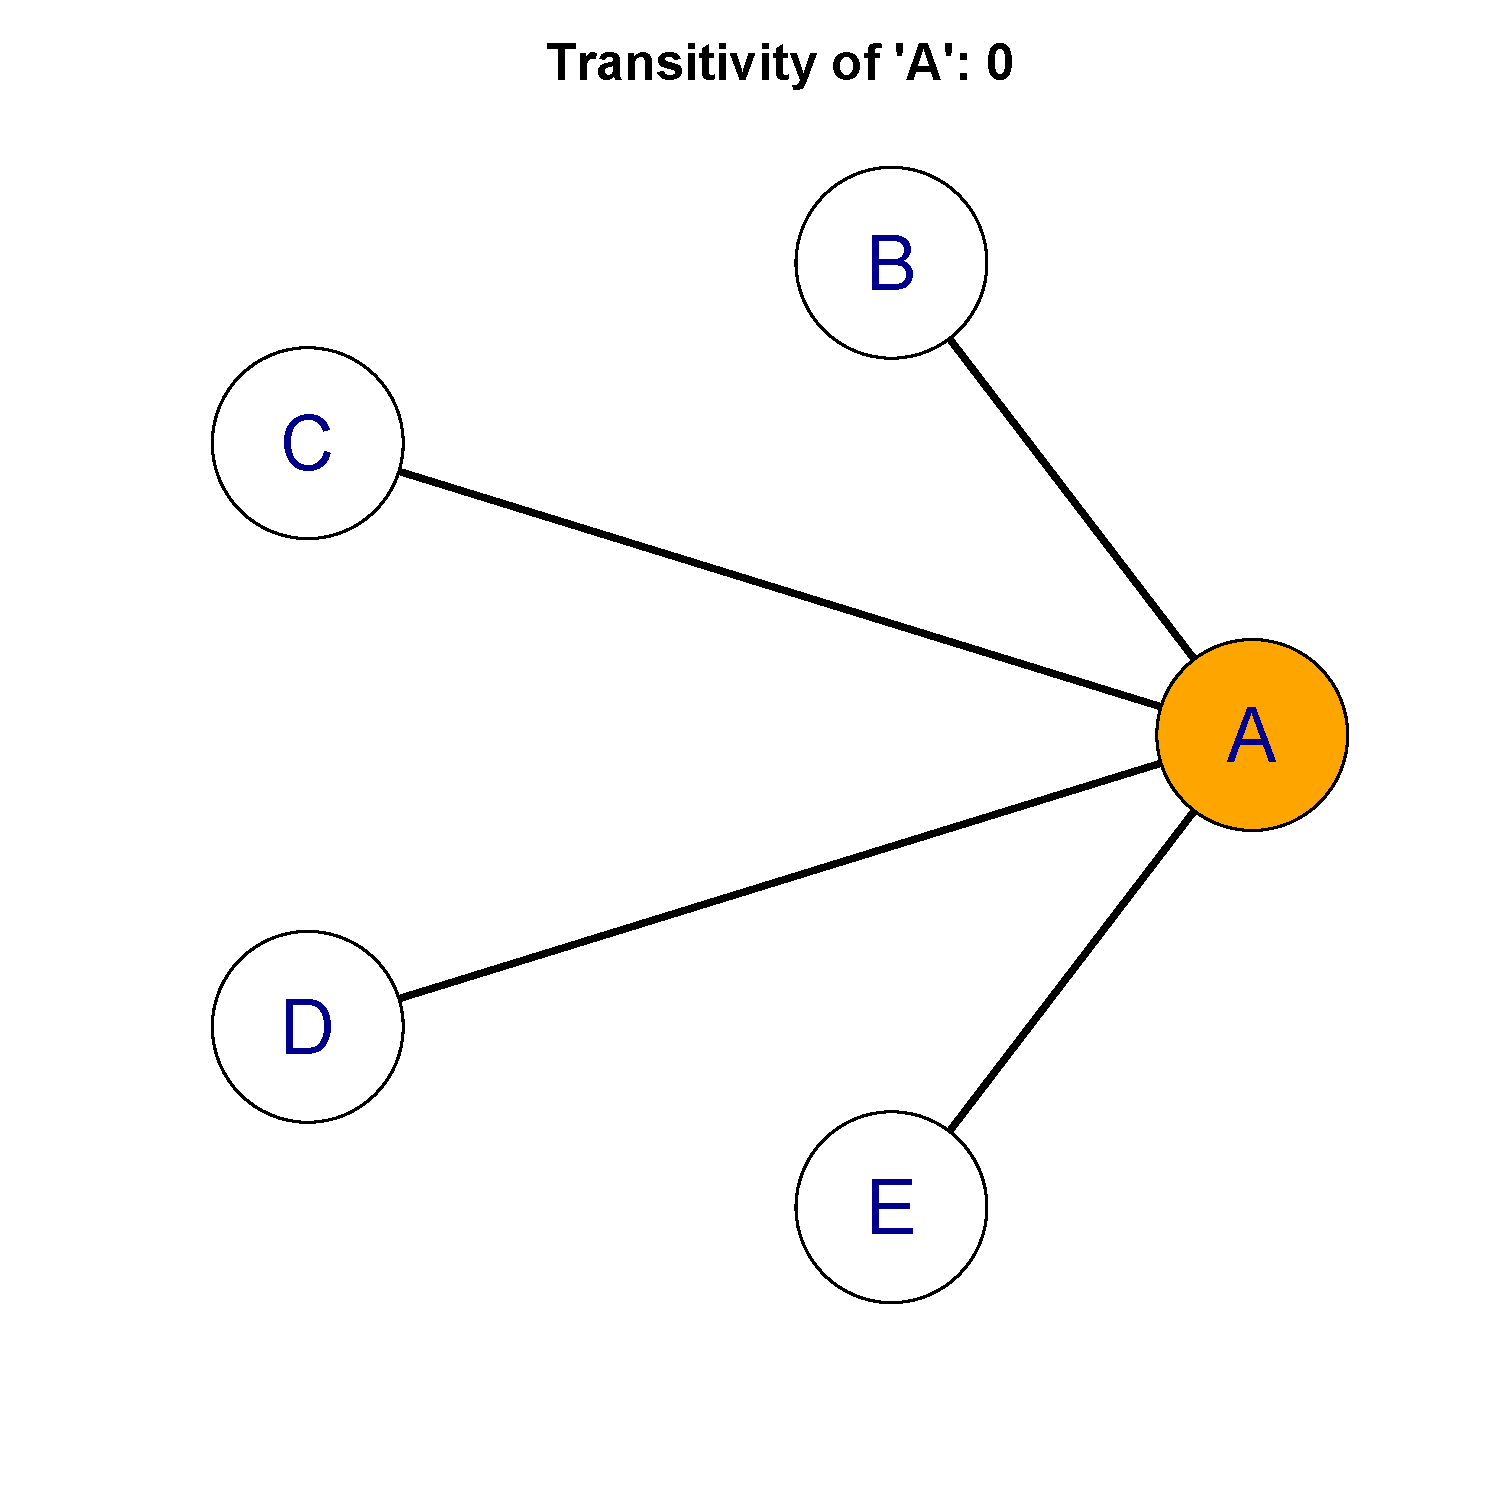
\includegraphics[width = 8.5cm]{BasicNetworkPlot1.pdf}
  	\end{figure}

\end{frame}

\begin{frame}[fragile]{Small Worlds with Focuses}

	\begin{figure}[h]
    \centering
  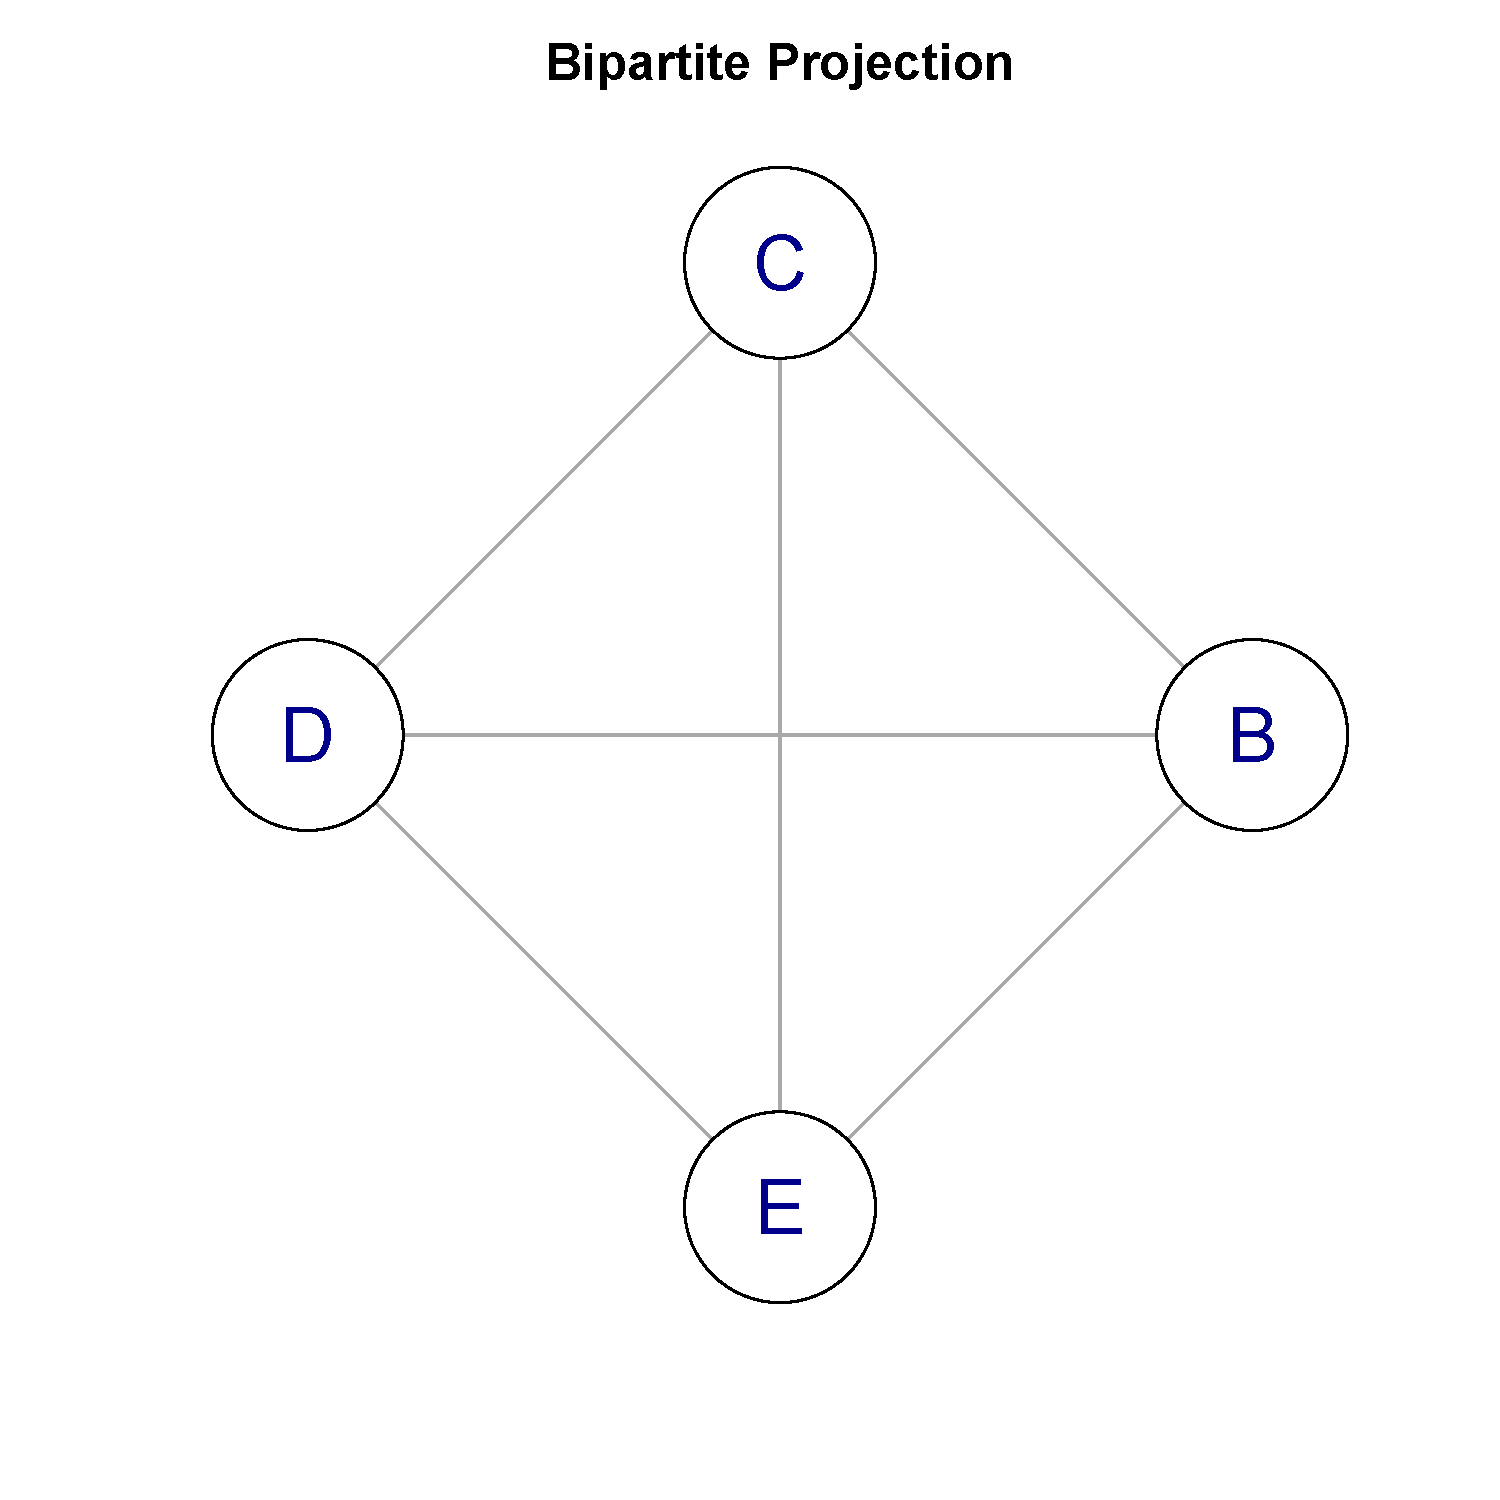
\includegraphics[width = 8.5cm]{BipartiteConcept.pdf}
  	\end{figure}

\end{frame}

\begin{frame}[fragile]{Small Worlds with Focuses}

	\begin{figure}[h]
    \centering
  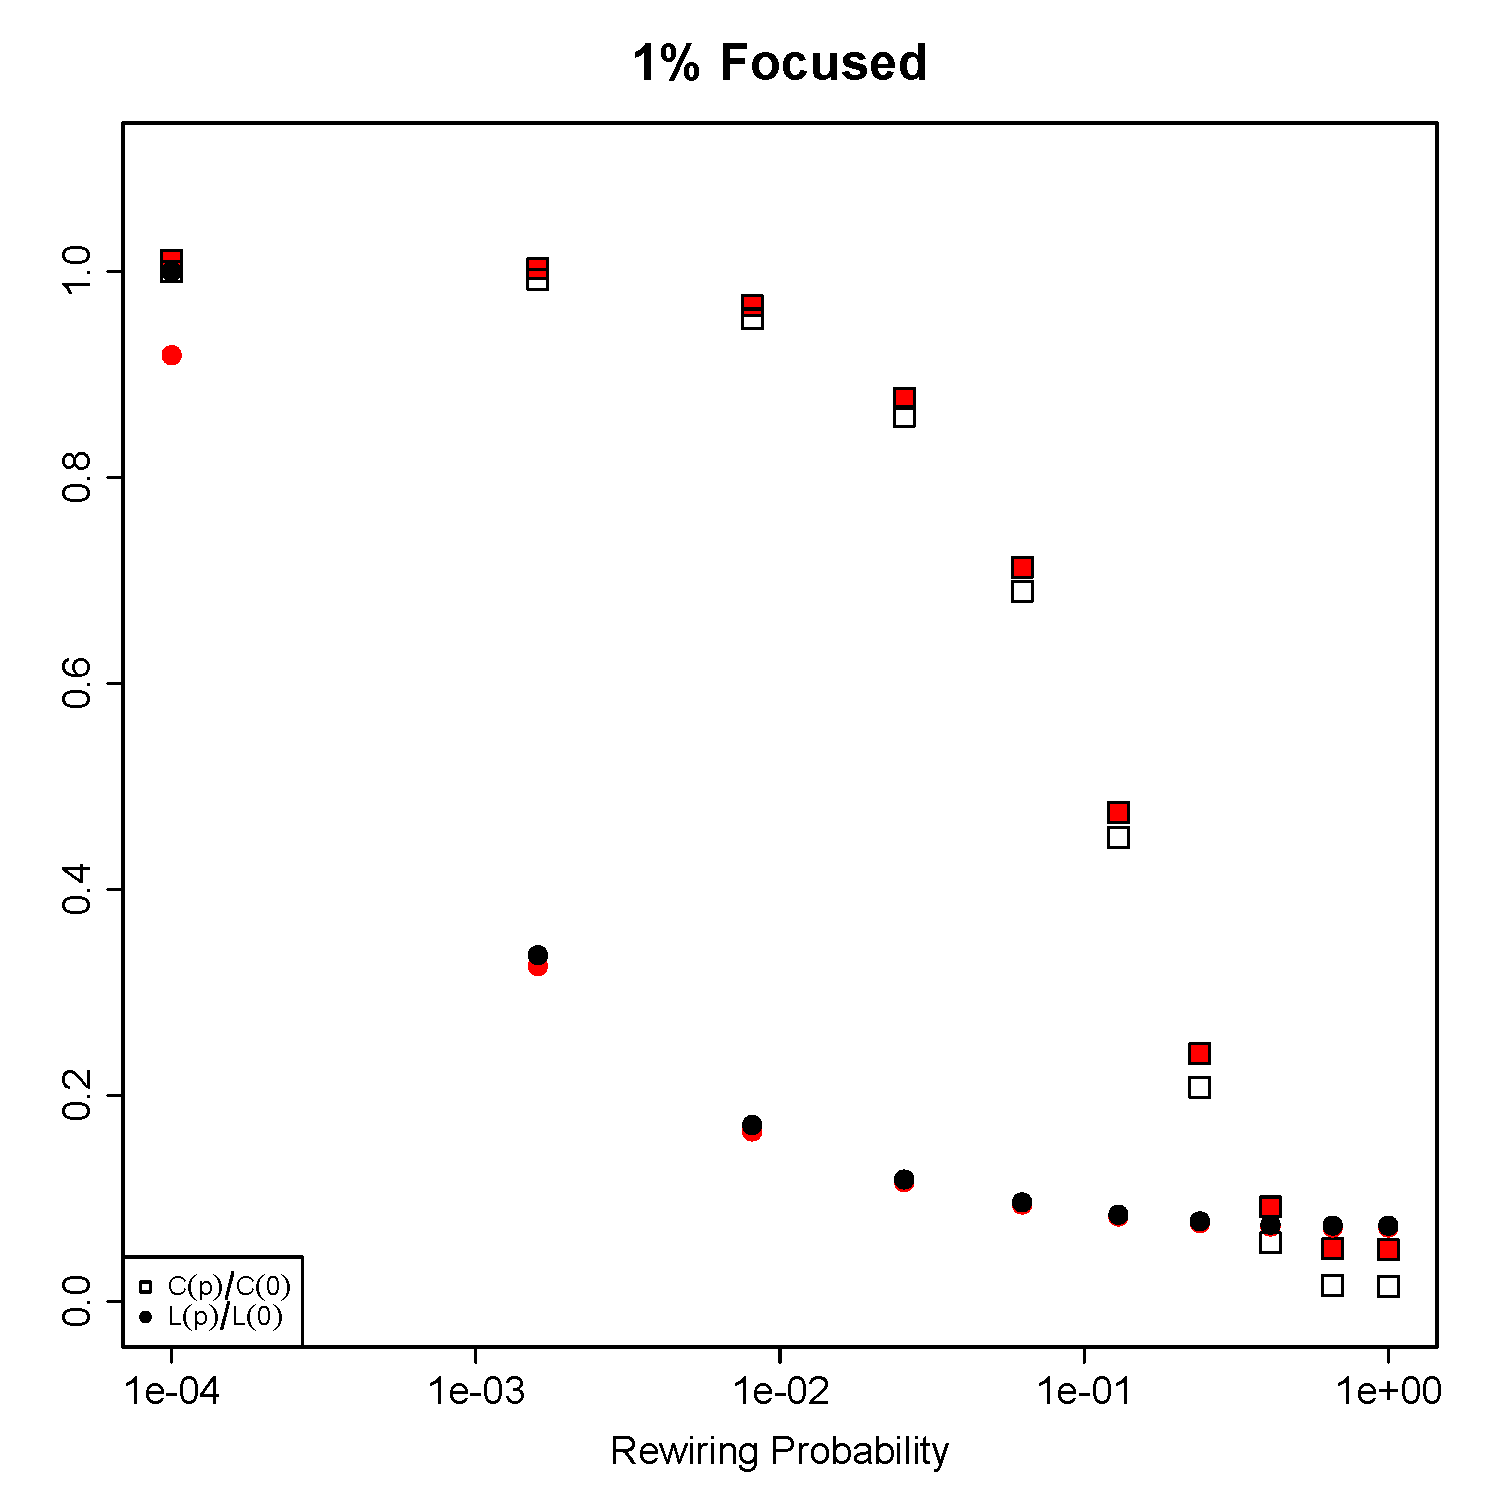
\includegraphics[width = 8.5cm]{FocusedWattsStrogatzPlot1.pdf}
  	\end{figure}

\end{frame}

\begin{frame}[fragile]{Small Worlds with Focuses}

	\begin{figure}[h]
    \centering
  \includegraphics[width = 8.5cm]{FocusedWattsStrogatzPlot2.pdf}
  	\end{figure}

\end{frame}

\begin{frame}[fragile]{Small Worlds with Focuses}

	\begin{figure}[h]
    \centering
  \includegraphics[width = 8.5cm]{FocusedWattsStrogatzPlot3.pdf}
  	\end{figure}

\end{frame}

\begin{frame}[fragile]{Small Worlds with Focuses}

	\begin{figure}[h]
    \centering
  \includegraphics[width = 8.5cm]{FocusedWattsStrogatzPlot4.pdf}
  	\end{figure}

\end{frame}

\appendix


\begin{frame}[allowframebreaks]{References}

  \bibliography{demo.bib}
  \bibliographystyle{apalike}

\end{frame}


\end{document}
